\documentclass[fleqn]{article}

\usepackage{enumerate}
\usepackage{amsmath}
\usepackage[letterpaper, margin=1in]{geometry}
\usepackage{tikz}
\usetikzlibrary{shapes,shapes.arrows,positioning}
\usepackage{pgfplots}

\begin{document}	
	\begin{enumerate}[{1}.1]
		\item \quad
		\begin{itemize}
			\item [9.]
			\begin{flalign*}
				C + R &= 9 && \\
				C - R &= 5 && \\
				2R &= 4 && \\
				R &= 2 && \\
				C - 2 &= 5 && \\
				C &= 5 &&
			\end{flalign*}
			
			\item [14.]
			\begin{alignat*}{4}
				&& J & {}+{} & S & {}={} && 20 + 4 \left( J - S \right) \\
				\Rightarrow && J & {}+{} & S & {}={} && 20 + 4J - 4S \\
				\Rightarrow && -3J & {}+{} & 5S & {}={} && 20
			\end{alignat*}
			\begin{alignat*}{3}
				&& 2S & {}={} && 40 + J \\
				\Rightarrow && -J + 2S & {}={} && 40
			\end{alignat*}
			\begin{alignat*}{4}
				&& -3J & {}+{} & 5S & {}={} & 20 & \\
				{}-{} 2( && -J & {}+{} & 2S & {}={} & 40 & ) \\
				\hline
				&& -J & {}+{} & S & {}={} & -60 &  \\
				\Rightarrow && & & S & {}={} & J - 60 &
			\end{alignat*}
			\begin{alignat*}{3}
				&& 2S & {}={} && 40 + J \\
				\Rightarrow && 2(J - 60) & {}={} && 40 + J \\
				\Rightarrow && 2J - 120 & {}={} && 40 + J \\
				\Rightarrow && J & {}={} && 160
			\end{alignat*}	
			\begin{alignat*}{3}
				& S & {}={} & J - 60 \\
				\Rightarrow & S & {}={} & 100
			\end{alignat*}
			
			\item [22.]
			\begin{alignat*}{4}
				&& A\left( 12T + 6C \right) + B\left( 8T + 4C \right) & {}={} && 48T + 24C \\
				\Rightarrow && 6A\left( 2T + C \right) + 4B\left( 2T + C \right) & {}={} && 24\left( 2T + C \right) \\
				\Rightarrow && 3A + 2B & {}={} && 12 \\	
			\end{alignat*}
			
			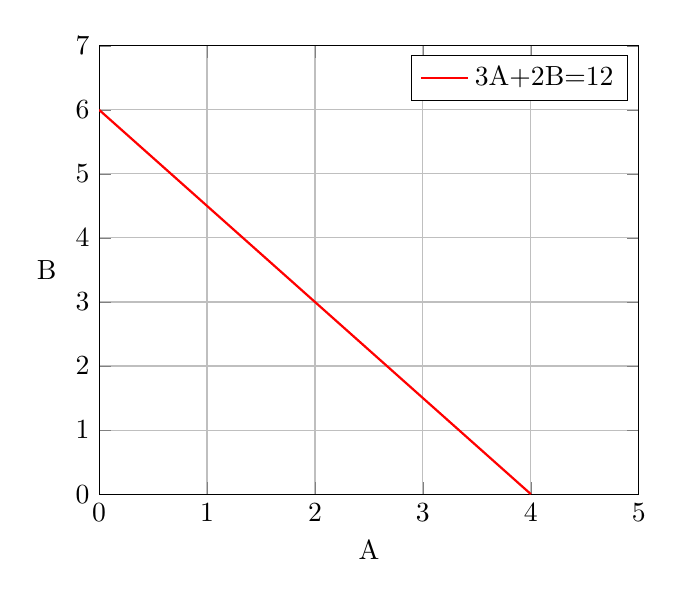
\begin{tikzpicture}[baseline={(current bounding box.north)}]
				\begin{axis} [
					xmin=0, xmax=5, xlabel=A, xtick distance=1,
					ymin=0, ymax=7, ylabel=B, ylabel style={rotate=-90}, ytick distance=1,
					domain=0:4,
					grid=major]
					\addplot [thick, color=red] {6-1.5*x};
					\addlegendentry{3A+2B=12}
				\end{axis}
			\end{tikzpicture} \\
			There are 3 integer pair solutions.
		\end{itemize}
		
		\item \quad
		\begin{itemize}
			\item [4.] \quad
			\begin{enumerate}[(a)]
				\item 
				\begin{alignat*}{4}
					R_1 & {}={} & 6H & {}+{} & 4D & {}+{} & 3G \\
					R_2 & {}={} & 3H & {}+{} & 6D & {}+{} & 2G \\
					R_2 & {}={} & 2H & {}+{} & 3D & {}+{} & 6G \\
					x_1R_1 + x_2R_2 + x_3R_3 & {}={} & 280H & {}+{} & 350D & {}+{} & 350G
				\end{alignat*}
				
				\item
				\begin{alignat*}{5}
					&& x_1R_1 + x_2R_2 + x_3R_3 & {}={} & 280H & {}+{} & 350D & {}+{} & 350G \\
					\Rightarrow && x_1\left( 6H + 4D + 3G \right) & & & & & & & \\
					&& + x_2\left( 3H + 6D + 2G \right) & & & & & & & \\
					&& + x_3\left( 2H + 3D + 6G \right) & {}={} & 280H & {}+{} & 350D & {}+{} & 350G \\
					\Rightarrow && H\left( 6x_1 + 3x_2 + 2x_3 \right) & & & & & & & \\
					&& + D\left( 4x_1 + 6x_2 + 3x_3 \right) & & & & & & & \\
					&& + G\left( 3x_1 + 2x_2 + 6x_3 \right) & {}={} & 280H & {}+{} & 350D & {}+{} & 350G 
				\end{alignat*}
				\begin{alignat*}{4}
					6x_1 & {}+{} & 3x_2 & {}+{} & 2x_3 & {}={} & 280\\
					4x_1 & {}+{} & 6x_2 & {}+{} & 3x_3 & {}={} & 350\\
					3x_1 & {}+{} & 2x_2 & {}+{} & 6x_3 & {}={} & 350
				\end{alignat*}
				\centering
				$\begin{array}{|c|c|c|c|c|c|}
					\hline
					x_1 & x_2 & x_3 & H & D & G \\
					\hline
					30 & 20 & 20 & 280 & 300 & 250 \\
					\hline
					25 & 25 & 25 & 275 & 325 & 275 \\
					\hline
					20 & 25 & 40 & 275 & 350 & 350 \\
					\hline
				\end{array}$
			\end{enumerate}
			
			\item [6.] \quad
			\begin{enumerate}[(a)]
				\item 
				\begin{alignat*}{4}
					J & {}={} & 10C & {}+{} & 1P & {}+{} & 30V \\
					F & {}={} & 50C & {}+{} & 3P & {}+{} & 10V \\
					M & {}={} & 200C & {}+{} & 0.2P & {}+{} & 0V \\
					x_1J + x_2F + x_3M & {}={} & 600C & {}+{} & 20P & {}+{} & 200V \\
				\end{alignat*}
			\end{enumerate}
		\end{itemize}
		
		\item \quad
		\begin{itemize}
			\item [3.] \quad
			\begin{itemize}
				\item [(c)]
				$p_2=0.25$, $p_3=0.25$, $p_4=0.5$, all other $p_i = 0$
				\begin{alignat*}{8}
					p'_1 & {}={} & 0.50p_1 & {}+{} & 0.25p_2 & & & & & & & & & {}={} && 0.0625 \\
					p'_2 & {}={} & 0.50p_1 & {}+{} & 0.50p_2 & {}+{} & 0.25p_3 & & & & & & & {}={} && 0.1875 \\
					p'_3 & {}={} & & & 0.25p_2 & {}+{} & 0.50p_3 & {}+{} & 0.25p_4 & & & & & {}={} && 0.3125 \\
					p'_4 & {}={} & & & & & 0.25p_3 & {}+{} & 0.50p_4 & {}+{} & 0.25p_5 & & & {}={} && 0.3125 \\
					p'_5 & {}={} & & & & & & & 0.25p_4 & {}+{} & 0.50p_5 & {}+{} & 0.50p_6 & {}={} && 0.125 \\
					p'_6 & {}={} & & & & & & & & & 0.25p_5 & {}+{} & 0.50p_6 & {}={} && 0
				\end{alignat*}
				
				\item [(d)]
				$p_1 = 0.1$, $p_2=0.2$, $p_3=0.2$, $p_4=0.2$, $p_5 = 0.2$, $p_6 = 0.1$
				\begin{alignat*}{8}
					p'_1 & {}={} & 0.50p_1 & {}+{} & 0.25p_2 & & & & & & & & & {}={} && 0.1 \\
					p'_2 & {}={} & 0.50p_1 & {}+{} & 0.50p_2 & {}+{} & 0.25p_3 & & & & & & & {}={} && 0.2 \\
					p'_3 & {}={} & & & 0.25p_2 & {}+{} & 0.50p_3 & {}+{} & 0.25p_4 & & & & & {}={} && 0.2 \\
					p'_4 & {}={} & & & & & 0.25p_3 & {}+{} & 0.50p_4 & {}+{} & 0.25p_5 & & & {}={} && 0.2 \\
					p'_5 & {}={} & & & & & & & 0.25p_4 & {}+{} & 0.50p_5 & {}+{} & 0.50p_6 & {}={} && 0.2 \\
					p'_6 & {}={} & & & & & & & & & 0.25p_5 & {}+{} & 0.50p_6 & {}={} && 0.1
				\end{alignat*}
			\end{itemize}
			
			\item [5.] \quad
			\begin{itemize}
				\item [(a)]
				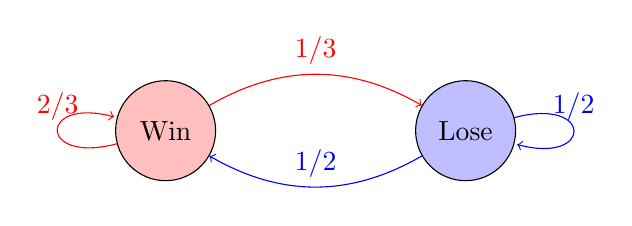
\begin{tikzpicture}[->, node distance=1.5in, baseline={(current bounding box.north)}]
					\centering
					\node [circle, draw, minimum size=0.5in, fill=red!25] (win) {Win};
					\node [circle, draw, minimum size=0.5in, fill=blue!25] (lose) [right of=win] {Lose};
					\path (win) edge [red] [loop left] node [above] {$2/3$} (win);
					\path (win) edge [red] [bend left] node [above] {$1/3$} (lose);
					\path (lose) edge [blue] [bend left] node [above] {$1/2$} (win);
					\path (lose) edge [blue] [loop right] node [above] {$1/2$} (lose);
				\end{tikzpicture}
				
				\item [(c)]
				$P(\text{winning the game after the next}) = \dfrac{2}{3} \times \dfrac{2}{3} + \dfrac{1}{3} \times \dfrac{1}{2} = \dfrac{11}{18}$
			\end{itemize}
			
			\item [8.] \quad
			\begin{enumerate}[(a)]
				\item
				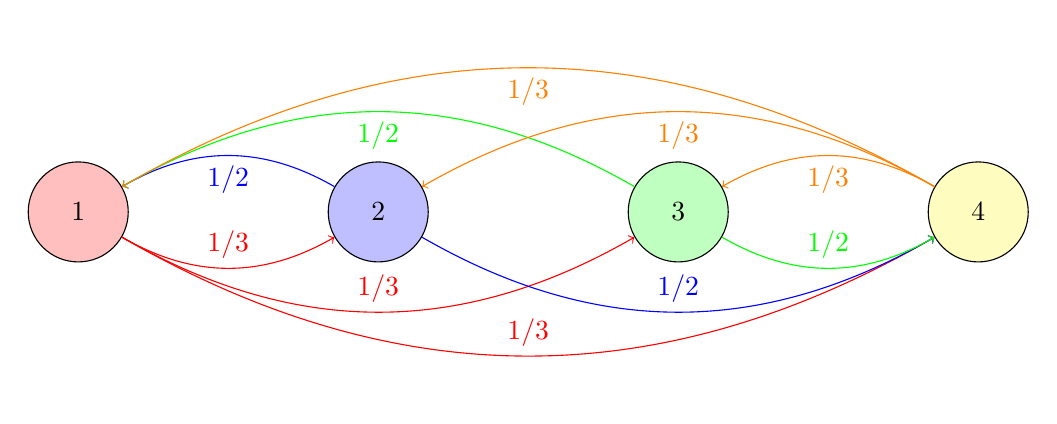
\begin{tikzpicture}[->, node distance=1.5in, baseline={(current bounding box.north)}]
					\centering
					\node [circle, draw, minimum size=0.5in, fill=red!25] (one) {1};
					\node [circle, draw, minimum size=0.5in, fill=blue!25] (two) [right of=one] {2};
					\node [circle, draw, minimum size=0.5in, fill=green!25] (three) [right of=two] {3};
					\node [circle, draw, minimum size=0.5in, fill=yellow!25] (four) [right of=three] {4};
					\path (one) edge [red] [bend right] node [above] {$1/3$} (two);
					\path (one) edge [red] [bend right] node [above] {$1/3$} (four);
					\path (one) edge [red] [bend right] node [above] {$1/3$} (three);
					\path (two) edge [blue] [bend right] node [below] {$1/2$} (one);
					\path (two) edge [blue] [bend right] node [above] {$1/2$} (four);
					\path (three) edge [green] [bend right] node [below] {$1/2$} (one);
					\path (three) edge [green] [bend right] node [above] {$1/2$} (four);
					\path (four) edge [orange] [bend right] node [below] {$1/3$} (one);
					\path (four) edge [orange] [bend right] node [below] {$1/3$} (two);
					\path (four) edge [orange] [bend right] node [below] {$1/3$} (three);
				\end{tikzpicture}
				
				\item
				Starting at room 1: \\
				$p_1=0$, $p_2=\dfrac{1}{3}$, $p_3=\dfrac{1}{3}$, $p_4=\dfrac{1}{3}$
				\begin{alignat*}{6}
					p'_1 & {}={} & & & \frac{1}{2}p_2 & {}+{} & \frac{1}{2}p_3 & {}+{} & \frac{1}{3}p_4 & {}={} & \frac{4}{9} \\
					p'_2 & {}={} & \frac{1}{3}p_1 & & & {}+{} & & & \frac{1}{3}p_4 & {}={} & \frac{1}{9} \\
					p'_3 & {}={} & \frac{1}{3}p_1 & & & {}+{} & & & \frac{1}{3}p_4 & {}={} & \frac{1}{9} \\
					p'_4 & {}={} & \frac{1}{3}p_1 & {}+{} & \frac{1}{2}p_2 & {}+{} & \frac{1}{2}p_3  & & & {}={} & \frac{3}{9}
				\end{alignat*}
				\begin{alignat*}{6}
					p''_1 & {}={} & & & \frac{1}{2}p'_2 & {}+{} & \frac{1}{2}p'_3 & {}+{} & \frac{1}{3}p'_4 & {}={} & \frac{6}{27} \\
					p''_2 & {}={} & \frac{1}{3}p'_1 & & & {}+{} & & & \frac{1}{3}p'_4 & {}={} & \frac{7}{27} \\
					p''_3 & {}={} & \frac{1}{3}p'_1 & & & {}+{} & & & \frac{1}{3}p'_4 & {}={} & \frac{7}{27} \\
					p''_4 & {}={} & \frac{1}{3}p'_1 & {}+{} & \frac{1}{2}p'_2 & {}+{} & \frac{1}{2}p'_3  & & & {}={} & \frac{7}{27}
				\end{alignat*}
				$P(\text{in room 4 after two periods})=\dfrac{7}{27}$
			\end{enumerate}
		\end{itemize}
	\end{enumerate}
\end{document}